\documentclass[10pt,a4paper]{article}
\usepackage{fontspec}
\setmainfont{PT Serif}\setsansfont{PT Sans}\setmonofont{PT Mono}[Scale=0.9]
\usepackage[russian]{babel}
\usepackage[a4paper,margin=1.5cm,top=1.3cm,bottom=1.5cm]{geometry}
\usepackage{amsmath,booktabs,graphicx,hyperref,enumitem}
\usepackage[font=small,skip=2pt]{caption}
\hypersetup{colorlinks,urlcolor=blue,linkcolor=black}
\setlist{nosep,leftmargin=1.2em}
\setlength{\parskip}{2pt}\setlength{\parindent}{0pt}
\renewcommand{\arraystretch}{1.05}
\newcommand{\code}[1]{\texttt{#1}}
\begin{document}
\sloppy

{\large\textbf{Экономика контекста, MCP-сервер, выбор из $N$ и петли}}\hfill Дорошенко Даниил, гр.\,507\\[1pt]
{\small Репозиторий с кодом, тестами, ноутбуком и сырыми логами: \url{https://github.com/Warlordg9/mcp-agent-tooling-lab}}

\section*{1. Теория: экономика контекста}
$C=\sum_{t=1}^{T}[\alpha(S+D)+ht]=\alpha(S+D)T+h\frac{T(T+1)}{2}\approx\alpha(S+D)T+\frac{hT^2}{2}$.
Приближения: $H_t\approx ht$ и $\sum_t t=\tfrac{T(T+1)}{2}\approx\tfrac{T^2}{2}$ (сумма заменена интегралом, отброшен член $hT/2$, ошибка $1/(T+1)\approx2{,}4\%$); история считается некэшируемой.
\textbf{(б)} $S{+}D=57\,000$, $hT^2/2=1{,}2$\,млн. При $\alpha=1$: $C=3\,480\,000$, история $34{,}5\%$; при $\alpha=0{,}1$: $C=1\,428\,000$, история $84{,}0\%$.
Теперь главный рычаг~--- $h$: $h\to h/2$ экономит $600$\,тыс. ($42\%$), а $D\to0$ лишь $220$\,тыс. ($15\%$), $\alpha\to0$~--- $228$\,тыс.
\textbf{(в)} A: $300N$, B: $500+5\cdot300=2000$; $300N>2000\Rightarrow N_{\min}=7$.
\textbf{(г)} B: $0{,}95\cdot0{,}90=0{,}855$; B перестаёт выигрывать при $A(N)\ge0{,}855$. Оптимизм для B: (1) кэш не учтён~--- статичный список A стоит $\alpha\cdot300N$, а меняющаяся выдача B ломает префикс (при $\alpha=0{,}1$ порог $N\ge67$), плюс лишний шаг поиска растит историю $h$; (2) Recall и $A(k)$ не независимы и не константы: top-5~--- самые похожие (трудные) кандидаты, ошибки поиска и выбора коррелированы, Recall падает с $N$.

\section*{2. MCP-сервер \code{consult\_mcp} (MCP 2026-07-28, \code{mcp==2.3.0}, \code{MCPServer})}
Домен~--- запись на консультации курса. 6 инструментов с префиксом \code{consult\_}: \code{search\_slots}, \code{get\_slot}, \code{book}, \code{get\_booking}, \code{list\_bookings}, \code{cancel}.
\textbf{Протокол:} только stateless-эра~--- \code{server/discover}, \code{\_meta} в каждом запросе, HTTP в режиме \code{stateless\_http}; \code{initialize} отклоняется ошибкой $-32022$, заголовка \code{Mcp-Session-Id} нет (тесты + Inspector \code{--protocol-era legacy}).
\textbf{Дизайн:} рукописные схемы (\code{enum} для формата, темы, преподавателя, статуса; \code{description} у каждого поля; \code{additionalProperties:\,false}~--- SDK по умолчанию его не ставит и пропускает лишние аргументы, поэтому middleware валидирует по нашей схеме); в каждом описании <<Используй, когда…>> и <<Не используй для…>>; \code{response\_format}: concise/detailed (detailed длиннее в $3{,}2$--$6{,}5$ раза, таблица в README).
\textbf{Ошибки}~--- результат с \code{isError:\,true} вида <<что не так. Как исправить: …>>. \textbf{Состояние}~--- только handle-аргументы \code{booking\_id}, \code{student\_id}, \code{cursor}; бронь видна новому экземпляру сервера.
\textbf{Проверка:} 19 тестов pytest (успех и ошибка на каждый инструмент, протокол, схемы), прогон MCP Inspector 2.10.1 CLI (\code{inspector/inspector\_log.txt}), CI на GitHub Actions.

\section*{3. Эксперимент}
\textbf{Протокол.} Модель \code{qwen2.5:3b} (Q4\_K\_M) через Ollama 0.40.2 на Apple M1 16\,ГБ; \code{temperature=0.7}, \code{seed=1..3}, \code{num\_ctx=16384} для всех $N$ (стандартные 4096 молча обрезали бы $N=100$); эмбеддинги \code{bge-m3}. Бюджет~--- \$0. \textbf{Пул} из 100 инструментов: 6 своих, 25 сгенерированных близких по смыслу (расписание, дедлайны, оценки, аудитории, календарь, поликлиника, экзамены) и 69 описаний инструментов публичных MCP-серверов (filesystem, git, github, slack, sqlite, memory, puppeteer, maps и др.; имена настоящие, тексты пересказаны). \textbf{30 запросов}: 24 к своим инструментам, 6 <<почти похожих>> (правильный~--- отвлекающий). Для запроса $S_N=\{\text{gold}\}\cup$ первые $N{-}1$ из перемешанного пула, $S_5\subset S_{20}\subset S_{50}\subset S_{100}$. A~--- все $N$ описаний со схемами в \code{tools}; B~--- top-5 из $S_N$ по косинусу эмбеддингов. Выбор~--- первый \code{tool\_call}; нет вызова или сбой~--- ошибка (полный знаменатель: $30\times3=90$ запусков на ячейку, сбоев 0, без вызова 19 из 720). Интервалы~--- 95\% перцентильный бутстрэп (10\,000) с ресэмплингом \emph{запросов} (точность запроса~--- среднее по 3 запускам).

\noindent\begin{minipage}[t]{0.46\textwidth}\vspace{0pt}
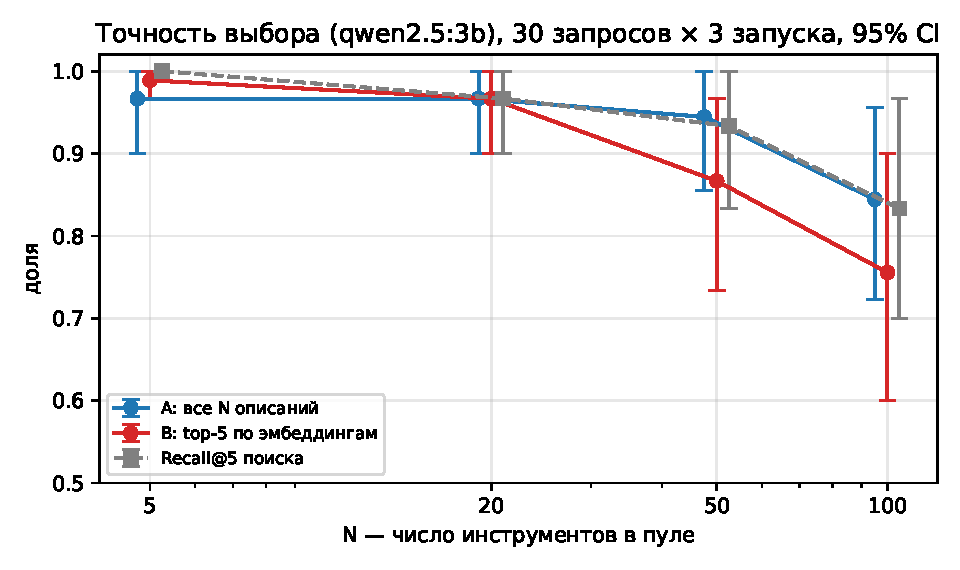
\includegraphics[width=\linewidth]{../experiment/results/accuracy_vs_N.pdf}
\captionof{figure}{Точность A и B и Recall@5 от $N$, 95\%~CI.}
\end{minipage}\hfill
\begin{minipage}[t]{0.52\textwidth}\vspace{2pt}\small
\captionof{table}{Часть A: точность и Recall@5, \% [95\% CI]; среднее число входных токенов на запрос (\code{prompt\_eval\_count}).}
\resizebox{\linewidth}{!}{\begin{tabular}{rcccrr}\toprule
$N$ & точность A & точность B & Recall@5 (B) & \multicolumn{2}{c}{вход. токенов: A / B} \\ \midrule
5 & 97 [90;\,100] & 99 [97;\,100] & 100 [100;\,100] & 750 & 750 \\
20 & 97 [90;\,100] & 97 [90;\,100] & 97 [90;\,100] & 1\,757 & 882 \\
50 & 94 [86;\,100] & 87 [73;\,97] & 93 [83;\,100] & 3\,993 & 1\,057 \\
100 & 84 [72;\,96] & 76 [60;\,90] & 83 [70;\,97] & 7\,734 & 1\,041 \\
\bottomrule\end{tabular}}\\[3pt]
\textbf{Итог A.} До $N=20$ оба варианта $\approx97\%$. Дальше A деградирует медленнее (84\% при $N=100$), а B ограничен сверху Recall@5 (83\%): если нужный инструмент найден, модель выбирает его в $91$--$93\%$ случаев. При $N\ge20$ B дешевле по входу в $2{,}0$--$7{,}4$ раза, но проигрывает $8$--$9$~п.п. при $N\ge50$ (интервалы перекрываются). Ошибки сосредоточены в своих близких инструментах (\code{list\_bookings}$\to$\code{cancel}, \code{get\_slot}$\to$\code{search\_slots}); <<почти похожие>> запросы почти всегда решены верно~--- секции <<Не используй>> работают.
\end{minipage}

\vspace{4pt}
\textbf{Часть B. Петли.} \code{consult\_search\_slots} в 50\% вызовов (монета с seed по задаче) отдаёт пустую строку; агент~--- тот же qwen2.5:3b, 6 инструментов через MCP-клиента, до 15 шагов, 20 задач <<запиши студента к преподавателю X по теме Y на дату или до даты Z>>; успех~--- активная бронь, удовлетворяющая условиям (проверка по состоянию сервера). LoopGuard: если пара (имя, аргументы) встречается $\ge3$ раз в окне последних 6 вызовов, вызов блокируется с сообщением; второе срабатывание завершает эпизод. Петля~--- $\ge3$ одинаковых вызова подряд или A-B-A-B. Кроме трёх требуемых условий добавлен контроль со стабильным инструментом.

\begin{center}\small
\captionof{table}{Часть B: доля эпизодов с петлёй и успеха, \% [95\% CI, бутстрэп по задачам]; средние шаги LLM и токены (вход+выход); режимы отказа~--- доля эпизодов.}
\resizebox{\textwidth}{!}{\begin{tabular}{lcccrrcc}\toprule
Условие (20 задач) & петля, \% & успех, \% & шагов & токенов & guard & выдуманный slot\_id & без брони \\ \midrule
пустой ответ, без LoopGuard & 5 [0;\,15] & 70 [50;\,90] & 5.2 & 14\,617 & 0 & 15\,\% & 15\,\% \\
пустой ответ + LoopGuard (3/6) & 5 [0;\,15] & 65 [45;\,85] & 5.2 & 14\,224 & 1 & 15\,\% & 20\,\% \\
ответ с подсказкой, без LoopGuard & 0 [0;\,0] & 60 [40;\,80] & 5.2 & 14\,325 & 0 & 10\,\% & 25\,\% \\
контроль: стабильный инструмент & 0 [0;\,0] & 75 [55;\,90] & 4.3 & 11\,681 & 0 & 0\,\% & 5\,\% \\
\bottomrule\end{tabular}}
\end{center}

\textbf{Что помогает сильнее.} В нашем прогоне~--- \emph{ни одно из двух} заметно: различия успеха ($60$--$70\%$) внутри интервалов. Слабая модель почти не зацикливается строго (1 эпизод из 20), LoopGuard сработал один раз. Пустой ответ ломает агента иначе: модель \emph{выдумывает} \code{slot\_id} (15\%) или заканчивает без брони; цена нестабильности относительно контроля~--- $-5$..$-15$~п.п. успеха и $+25\%$ токенов. <<Исправленный>> ответ <<ничего не найдено; попробуйте другое значение date>> на деле \emph{ложен} (слоты есть, это сбой), поэтому модель чаще меняет дату и сдаётся (без брони 25\%). Вывод: исправлять надо инструмент, но правдиво (<<временная ошибка, повторите запрос>> или ретрай на стороне сервера); guard в harness~--- страховка от редкого, но дорогого случая (эпизод с петлёй стоил 37\,тыс. токенов против 14\,тыс. в среднем), а не замена честного сообщения.

\textbf{Угрозы валидности.}
(1) \emph{Малая выборка и одна модель:} 30 запросов и 20 задач по 1 эпизоду дают широкие интервалы; результаты 3B-модели в Q4 не обязаны переноситься на крупные модели: у них соотношение петель, выдумывания и отказов может быть другим.
(2) \emph{Конструкция пула и разметки:} запросы и <<близкие>> отвлекающие написаны автором, описания публичных серверов пересказаны по памяти и короче своих; эмбеддинги видят только описание; разметка одним человеком. Поиск в B использует исходный запрос, а не переформулировку агентом~--- это оптимистично для B.
(3) \emph{Измерение токенов и харнесс:} \code{prompt\_eval\_count} считает весь промпт, но не учитывает кэш префикса (по стоимости A с кэшем дешевле, чем в таблице); системный промпт части B подсказывает порядок шагов (без него модель останавливалась после поиска); реализация LoopGuard по описанию из задания, а не по коду лекции.

\end{document}
